\section{Experimental Setup}

    \subsection*{Circuit components}
    \begin{enumerate}
        \item 2 Transistors (CL100 or equivalent)
        \item Power supply
        \item 10 resistors of various specifications
        \item 4 Capacitors 
        \item Function Generator
        \item Oscilloscope
        \item Multimeters
        \item Connecting wires
        \item Breadboard
    \end{enumerate}

    \subsection*{Circuit Diagram}
    \begin{figure}[H]
        \centering
        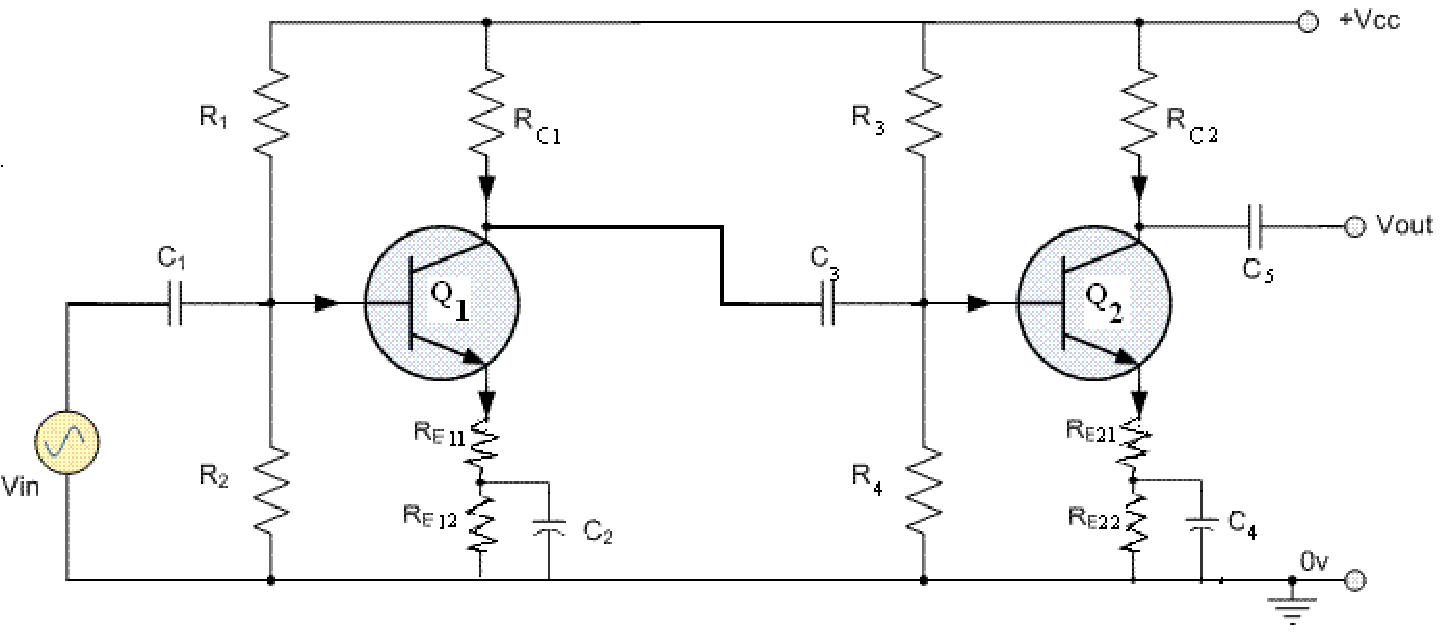
\includegraphics[width=1\columnwidth]{images/f1.png}
        \caption{Circuit diagram for the setup.}
        \label{fig:1}
    \end{figure}

\section{Observations}

\begin{table}[H]
    \centering
    \begin{tabular}{ll}
    \hline
    \textbf{Stage 1} (Q$_1$)  & \textbf{Stage 2} (Q$_2$)  \\ \hline
    $\beta_1 = 189$ & $\beta_2 = 184$ \\
    $R_1 = 26.48\,k\Omega$ & $R_3 = 27.16\,k\Omega$ \\
    $R_2 = 4.900\,k\Omega$ & $R_4 = 4.918\,k\Omega$ \\
    $R_{C1} = 3.835\,k\Omega$ & $R_{C2} = 3.843\,k\Omega$ \\
    $R_{E11} = 0.590\,k\Omega$ & $R_{E21} = 0.559\,k\Omega$ \\
    $R_{E12} = 0.466\,k\Omega$ & $R_{E22} = 0.469\,k\Omega$ \\
    $C_{1} = 1.036\,\mu$F & $C_{4} = 83.1\,\mu$F \\
    $C_{2} = 1.014\,\mu$F & $C_{5} = 99.0\,\mu$F \\
    \hline
    \end{tabular}
    \label{tab:1}
\end{table}

\begin{itemize}
    \item $V_{CC} = 12$ V
    \item $V_i$ (pp) = 200 mV
    \item $C_3 = 0.986\,\mu$F\\
\end{itemize}

We measured the following values from the D.C. analysis of the circuit.

\begin{table}[H]
    \centering
    \begin{tabular}{|c|c|c|c|c|}
    \hline
     & \multicolumn{2}{|c|}{Stage 1 (Q$_1$)} & \multicolumn{2}{|c|}{Stage 2 (Q$_2$)} \\ \hline
    Parameter & Computed  & Observed  & Computed  & Observed\\
     &  Value &  Value &  Value &  Value\\ \hline
    $V_B$ (V) & 1.874  &  1.835 & 1.839  &  1.808 \\
    $V_E$ (V) & 1.174  &  1.236 & 1.139  &  1.214 \\
    $I_C\approx I_E$ (mA) & 1.11 & 1.17 & 1.11  &  1.17 \\
    $V_{CE}$ (V) & 6.57 & 6.26 & 1.59  &  1.26 \\
    \hline
    \end{tabular}
    \caption{D.C. analysis of the circuit}
    \label{tab:2}
\end{table}

From this, the Q-point of stage is the found to be (6.26 V, 1.17 mA) and that of stage 2 is found to be (6.26 V, 1.17 mA).

The mid-frequency voltage gain ($V_o/V_i$) (at $f \approx 20$ kHz) was measured as follows.

\begin{table}[H]
    \centering
    \begin{tabular}{|c|c|c|c|c|}
    \hline
     & \multicolumn{2}{|c|}{Stage 1 (Q$_1$)} & \multicolumn{2}{|c|}{Stage 2 (Q$_2$)} \\ \hline
    Parameter & Computed  & Observed  & Computed  & Observed\\
     &  Value &  Value &  Value &  Value\\ \hline
    Unloaded  & \multirow{1}{*}{6.26}  &  \multirow{1}{*}{5.95} & \multirow{1}{*}{6.61}  &  \multirow{1}{*}{6.40} \\
    Voltage Gain        & (15.93 dB)   & (15.49 dB)             & (15.94 dB)          &  (16.12 dB) \\ \hline
    Loaded & \multirow{1}{*}{2.19} & \multirow{1}{*}{3.50} & \multirow{2}{*}{-}  &  \multirow{2}{*}{-} \\
    Voltage Gain& (6.81 dB) & (10.88 dB)  & &   \\
    \hline
    \end{tabular}
    \caption{Mid-frequency voltage gain at $\sim$20 kHz}
    \label{tab:3}
\end{table}

\section{Calculations \& Data Analysis}

\subsection*{Input and Output Impedances}
For stage 1, $r_{e_1}=26$mV$/I_{E1}=26\text{ mV}/1.17\text{ mA}=22.22\,\Omega$. Therefore,
\begin{align*}
    Z_{i1} &= R_1 \parallel R_2 \parallel \beta_1 r_{e1}\\
    &= \left( \frac{1}{26480} + \frac{1}{4900} + \frac{1}{189 \times 22.22} \right)^{-1}\\
    &= 2.083\,k\Omega
\end{align*}

And output impedance,
\begin{align*}
    Z_{o1} &= R_{C1} \parallel r_{o1} \\
    &= \left( \frac{1}{R_{C1}}+\frac{1}{r_{o1}}\right)^{-1} \\
    &\approx R_{C1}=3.835\,\text{k}\Omega
\end{align*}
Since $r_o$ is is the range of $\sim$ 100 k$\Omega$, we can ignore it.

Similarly for stage 2, $r_{e_2}=26$mV$/I_{E2}=22.22\,\Omega$. Therefore,
\begin{align*}
    Z_{i2} &= R_3 \parallel R_4 \parallel \beta_2 r_{e_2}\\
    &= \left( \frac{1}{27160} + \frac{1}{4918} + \frac{1}{184 \times 22.22} \right)^{-1}\\
    &= 2.062\,k\Omega
\end{align*}

And output impedance,
\begin{align*}
    Z_{o2} &= R_{C2} \parallel r_{o_2} \\
    &= \left( \frac{1}{R_{C2}}+\frac{1}{r_{o2}}\right)^{-1} \\
    &\approx R_{C2}=3.843\,\text{k}\Omega
\end{align*}

\subsection*{Mid-frequency Gain}

Using Eqs. (4) and (5), loaded gain of the first stage

\begin{align*}
    A_{V_1} &= \frac{R_{C1} \parallel Z_{i2}}{R_{E1} + r_{e1}}\\
    &=\frac{\left( \frac{1}{3835} + \frac{1}{2062}\right)^{-1}}{590+22.22}\\
    &= 2.19\,\,(\text{or 6.81 dB})
\end{align*}

unloaded gain of first stage,
\begin{align*}
    A'_{V_1} &= \frac{R_{C1}}{R_{E1} + r_{e1}}\\
    &=\frac{3835}{590+22.22}\\
    &= 6.26\,\,(\text{or 15.94 dB})
\end{align*}

unloaded gain of second stage,
\begin{align*}
    A_{V_2} &= \frac{R_{C2}}{R_{E1} + r_{e1}}\\
    &=\frac{3843}{559.3+22.22}\\
    &= 6.61\,\,(\text{or 16.40 dB})
\end{align*}

The overall computed gain of the 2 stage amplifier,

\begin{align*}
    A_{V_\text{comp}}=A_{V1}\times A_{V2} = 14.48\,\,(\text{or 23.21 dB})
\end{align*}

Observed value of total gain,
\begin{align*}
    A_{V_\text{obs}} = 19.75\,\,(\text{or }25.91\,\text{dB})
\end{align*}

\subsection*{Frequency Response Curve}

Here is the plot of the frequency response curve of the circuit.
\begin{figure}[H]
    \centering
    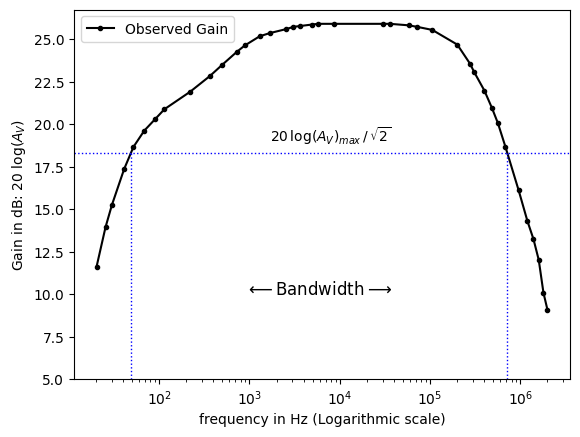
\includegraphics[width=1\columnwidth]{images/g1.png}
    \caption{Frequency response curve: $A_V$ vs. frequency plot}
    \label{graph}
\end{figure}

From Fig. \ref{graph}, we can estimate the following values,

\begin{itemize}
    \item Mid frequency Gain: 25.91 dB (or $V_o/V_i=19.75$)
    \item Cut-off frequencies: 48.46 Hz and 712.89 kHz and 
    \item Bandwidth: 712.83 kHz\\
\end{itemize}